\documentclass[11pt]{beamer}
\usetheme{Warsaw}
\usepackage[utf8]{inputenc}
%\usepackage[magyar]{babel}
\usepackage[T1]{fontenc}
\usepackage{amsmath}
\usepackage{amsfonts}
\usepackage{amssymb}
\usepackage{graphicx}
\usepackage{xurl}
\usepackage{multimedia}
\usepackage{xurl}
\newenvironment{trienv}{\only{\setbeamertemplate{items}[triangle]}}{}
\newenvironment{squareenv}{\only{\setbeamertemplate{items}[square]}}{}
\author{Bendegúz Borkovits T7UR9P}
\title{Simulating detectors with Geant4 4th presentation}
%\setbeamercovered{transparent} 
\setbeamertemplate{navigation symbols}{\insertframenumber/\inserttotalframenumber} 
%\logo{} 
\institute{Scientific Modeling Computer Laboratory} 
\date{April 2022} 
%\subject{} 
\begin{document}


\begin{frame}
\titlepage
\end{frame}

\begin{frame}{Previously...}
    \begin{itemize}
        \item<tri@1-> Properties and structure of NEBULA detector.
        \vspace{0.2 cm}
        \item<tri@1-> Failed to install smsimulator.
        \vspace{0.2 cm}
        \item<tri@1-> Problems with launching Balázs Pál simulation.
        \vspace{0.2 cm}
    \end{itemize}
    \centering
    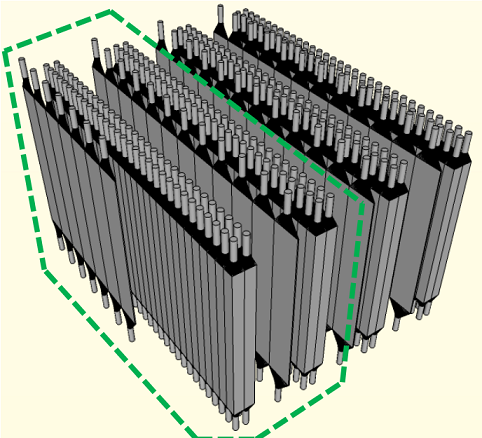
\includegraphics[scale = 0.6]{walls.png}
\end{frame}

\begin{frame}{Crisis averted!}
    \begin{itemize}
        \item<tri@1-> Out of 60 NEUT modules per wall, now only 20 rods are simulated and as 1 wall.
        \vspace{0.2 cm}
    \end{itemize}
    \centering
    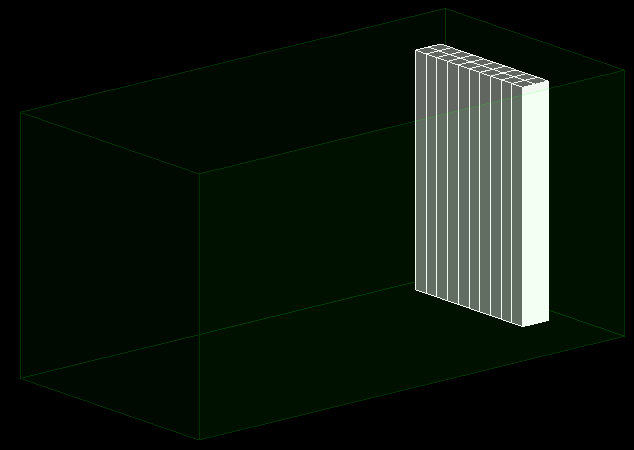
\includegraphics[scale = 0.76]{neut.png}
\end{frame}

\begin{frame}{Neutron beam}
        \begin{itemize}
        \item<tri@1-> 100 uniformly distributed neutrons, each has 100 MeV energy.
        \vspace{0.2 cm}
        \item<tri@1-> Many particles are difficult to visualize properly.
        \vspace{0.2 cm}
    \end{itemize}
    \centering
    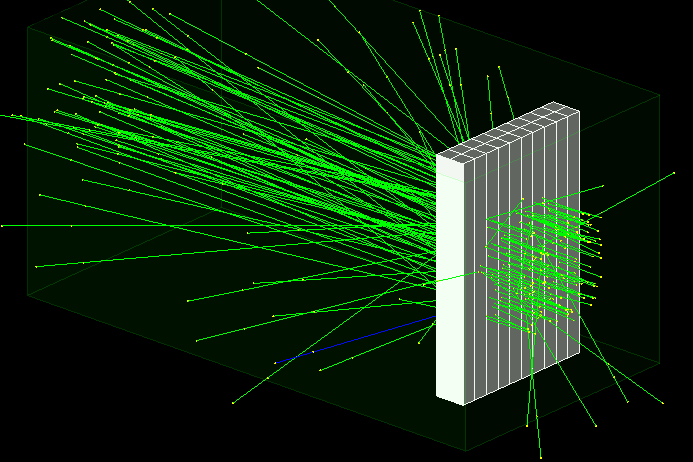
\includegraphics[scale = 0.68]{qbbc_neutbeam.png}
\end{frame}

\begin{frame}{Physics lists}
    \begin{itemize}
        \item<tri@1-> QBBC: Geant4 Bertini and Binary cascade models
        \vspace{0.2 cm}
        \item<tri@1-> QGSP: Quark Gluon String model for high energy hadronic interactions of protons, neutrons, pions, and Kaons
        \vspace{0.2 cm}
        \begin{itemize}
            \item<square@1-> QGSP\_BERT\_HP: Geant4 Bertini cascade, data driven high precision neutron package (HP)
            \vspace{0.2 cm}
            \item<square@1-> QGSP\_BIC\_HP: Geant4 Binary cascade, binary light ion cascade
            \vspace{0.2 cm}
            \item<square@1-> QGSP\_INCLXX: Liege Intranuclear Cascade model
            \vspace{0.2 cm}
            \item<square@1-> QGSP\_INCLXX\_HP: Improved version of the previous one
        \end{itemize}
    \end{itemize}
\end{frame}

\begin{frame}{Relative number of particles (particle types)}
    \centering
    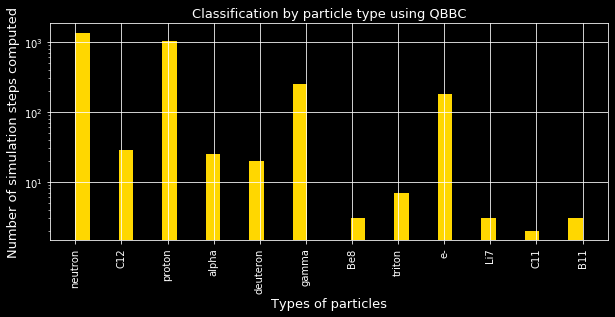
\includegraphics[scale = 0.46]{classpart.png}
    \begin{itemize}
    \vspace{0.2 cm}
        \item<tri@1-> Most particles: neutrons and protons.
        \vspace{0.2 cm}
        \item<tri@1-> Many by-products with lesser relevance.
        \vspace{0.2 cm}
        \item<tri@1-> Complete figure: \url{https://github.com/borbende/Scientific-Modelling-Computer-lab/blob/main/postmidterm2/figures/numparticles.png}
    \end{itemize}
\end{frame}

\begin{frame}{Relative number of particles (process types)}
    \centering
    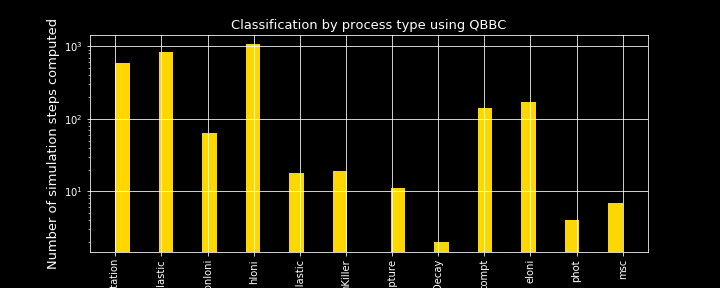
\includegraphics[scale = 0.46]{classproc.png}
    \begin{itemize}
    \vspace{0.2 cm}
        \item<tri@1-> Hadronic processes are dominant (neutrons, protons).
        \vspace{0.2 cm}
        \item<tri@1-> Difficult to filter out Geant4 process names.
        \vspace{0.2 cm}
        \item<tri@1-> Complete figure: \url{https://github.com/borbende/Scientific-Modelling-Computer-lab/blob/main/postmidterm2/figures/numprocess.png}
    \end{itemize}
\end{frame}

\begin{frame}{Relative number of particles (volume types)}
    \centering
    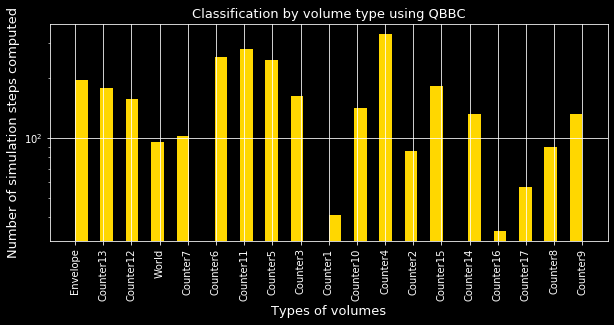
\includegraphics[scale = 0.46]{classvol.png}
    \begin{itemize}
    \vspace{0.2 cm}
        \item<tri@1-> The counters are the NEUT modules.
        \vspace{0.2 cm}
        \item<tri@1-> Fewer on the sides of the wall.
        \vspace{0.2 cm}
        \item<tri@1-> Complete figure: \url{https://github.com/borbende/Scientific-Modelling-Computer-lab/blob/main/postmidterm2/figures/numvolumes.png}
    \end{itemize}
\end{frame}

\begin{frame}{Distribution of energy (particle type)}
        \centering
    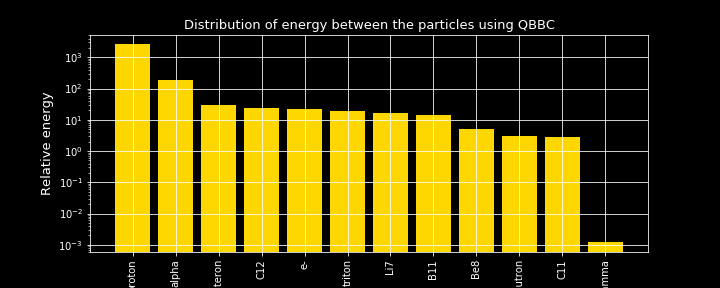
\includegraphics[scale = 0.46]{prenpart.png}
    \begin{itemize}
    \vspace{0.2 cm}
        \item<tri@1-> Protons deposited the largest amount of energy.
        \vspace{0.2 cm}
        \item<tri@1-> Third figure in the complete set is bugged.
        \vspace{0.2 cm}
        \item<tri@1-> Complete figure: \url{https://github.com/borbende/Scientific-Modelling-Computer-lab/blob/main/postmidterm2/figures/enpart.png}
    \end{itemize}
\end{frame}

\begin{frame}{Distribution of energy (process type)}
        \centering
    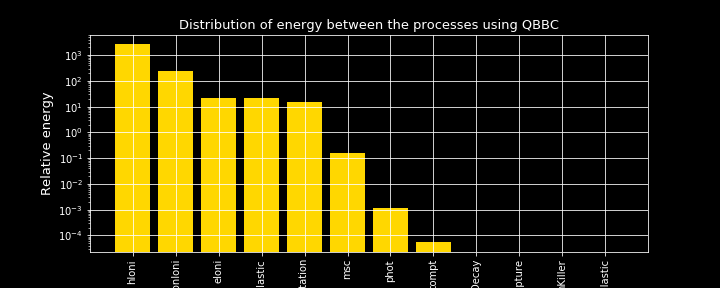
\includegraphics[scale = 0.46]{prenproc.png}
    \begin{itemize}
    \vspace{0.2 cm}
        \item<tri@1-> Hadronic ionization dominates.
        \item<tri@1-> Differences are too large even for log scale.
        \item<tri@1-> Complete figure: \url{https://github.com/borbende/Scientific-Modelling-Computer-lab/blob/main/postmidterm2/figures/enproc.png}
    \end{itemize}
\end{frame}

\begin{frame}{Distribution of energy (volume type)}
        \centering
    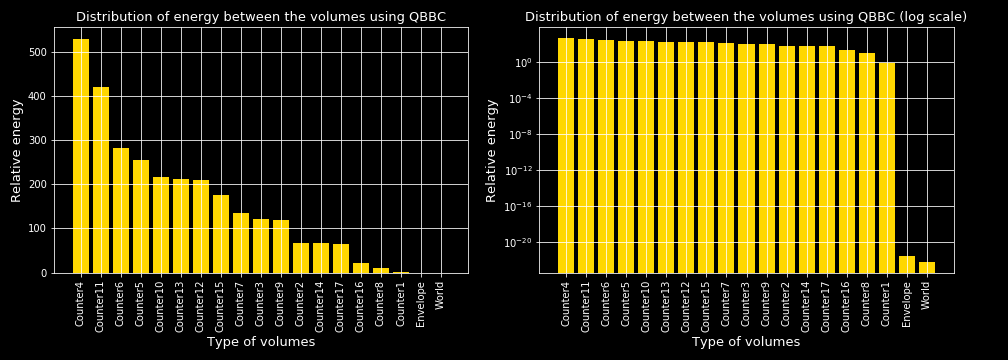
\includegraphics[scale = 0.33]{prenvol.png}
    \begin{itemize}
    \vspace{0.2 cm}
        \item<tri@1-> Lower energy deposited on the sides of the wall.
        \vspace{0.2 cm}
        \item<tri@1-> Barely any energy in the enveloping volumes.
        \vspace{0.2 cm}
        \item<tri@1-> Complete figure: \url{https://github.com/borbende/Scientific-Modelling-Computer-lab/blob/main/postmidterm2/figures/envol.png}
    \end{itemize}
\end{frame}

\begin{frame}{Final steps}
    \begin{itemize}
        \item<tri@1-> Simulation stands ready.
        \vspace{0.2 cm}
        \item<tri@1-> Outputs show promise.
        \vspace{0.2 cm}
        \item<tri@1-> Easy way of changing input energy.
        \vspace{0.2 cm}
        \item<square@1-> Change the energy between 100-300 MeV.
        \vspace{0.2 cm}
        \item<square@1-> Include extra particles?
        \vspace{0.2 cm}
        \item<square@1-> Measure detector efficiency?
    \end{itemize}
\end{frame}

\begin{frame}{Sources}
\begin{itemize}
        \item<tri@1-> Geant4 documentation: \url{https://geant4.web.cern.ch/}
        \vspace{0.3 cm}
        \item<tri@1-> NEBULA detector official site: \url{http://be.nucl.ap.titech.ac.jp/~nebula/index.php}
        \vspace{0.3 cm}
        \item<tri@1-> Balázs Pál simulation: \url{https://github.com/masterdesky/ELTE_Modelling_Lab_2021/tree/main/project/project_nebula/NEBULA}
        \vspace{0.3 cm}
        \item<tri@1-> My github: \url{https://github.com/borbende/Scientific-Modelling-Computer-lab/tree/main/postmidterm2}
\end{itemize}
\end{frame}




\end{document}
